\documentclass[11pt,a4paper]{article}
\usepackage[utf8]{inputenc}
\usepackage[T1]{fontenc}
\usepackage[french]{babel}
\usepackage{lmodern}
\usepackage[margin=2.1cm]{geometry}
\usepackage{graphicx}
\usepackage{booktabs}
\usepackage{tabularx}
\usepackage{float}
\usepackage{caption}
\usepackage{xcolor}
\usepackage[hidelinks]{hyperref}
\usepackage{enumitem}
\setlist{itemsep=1pt,topsep=3pt}
\graphicspath{{figures/}}
\captionsetup{font=small,labelfont=bf}

\title{\textbf{Prédire un revenu supérieur à 50\,000\,\$ :\\une preuve de concept d'apprentissage supervisé}\\[4pt]
\large Supervised Learning \& Model Engineering (MSA-DATB09-04)}
\author{Jérémy Caillaud \and Yanis Rajhi \and Hugo van Zuylen}
\date{Octobre 2026}

\begin{document}
\maketitle

\begin{center}
\fbox{\begin{minipage}{0.92\textwidth}
\textbf{Dataset : Adult / Census Income} (OpenML, version 2, \texttt{fetch\_openml(name="adult", version=2)}).\\
\textbf{Dépôt Git :} \url{https://github.com/CLDprog/Supervised-Learning-Census-Income-}\\
\textbf{Modèle final :} Gradient Boosting réglé avec Optuna, sans pondération des classes, seuil 0,404.
\textbf{Test} (ouvert une seule fois) : AP 0,833, ROC-AUC 0,931, F1 0,734, Brier 0,087.
\end{minipage}}
\end{center}

%=====================================================================
\section{Problème et cadrage}

Le recensement américain de 1994 décrit 48\,842 personnes par 14 variables (âge, diplôme, profession, statut marital, heures travaillées, plus-values\ldots). La cible indique si le revenu annuel dépasse 50\,000\,\$. Nous traitons une \textbf{classification binaire} dont la classe positive, \texttt{>50K}, ne représente que \textbf{23,9\,\%} des personnes.

\paragraph{Cas d'usage.} Un analyste socio-économique veut estimer, à partir des réponses au recensement, si une personne appartient à la catégorie des hauts revenus. Il s'agit de classer une catégorie de revenu observée, pas de prévoir un salaire futur ; le modèle n'est pas destiné à des décisions individuelles. Aucun coût monétaire n'étant attribué aux erreurs, le \textbf{F1 de la classe \texttt{>50K}} arbitre entre précision et rappel.

\paragraph{Métriques.} Un modèle qui répond toujours \texttt{<=50K} obtient 76\,\% d'accuracy avec un rappel nul : l'accuracy est donc écartée comme critère. La \textbf{métrique principale est l'Average Precision} (AP), qui résume le compromis précision/rappel sur tous les seuils. Nous rapportons aussi ROC-AUC, précision, rappel, F1 et matrice de confusion, identiques pour tous les modèles (fonction commune \texttt{evaluate\_model}).

\paragraph{Protocole de validation.} Après suppression de 52 doublons exacts (48\,790 lignes), les données sont découpées en \textbf{70\,/\,15\,/\,15} (34\,156 / 7\,317 / 7\,317), stratifié sur la cible, graine 42. Cinq paires de profils identiques à étiquettes opposées sont gardées dans la même partition, pour qu'aucune copie d'un profil ne traverse la frontière train/test. Chaque partition est protégée par une empreinte SHA-256.
\begin{itemize}
\item \textbf{Train} : apprentissage, validation croisée \emph{groupée} en 5 découpages (\texttt{StratifiedGroupKFold}), réglage Optuna.
\item \textbf{Validation} : choix des seuils de décision et des réglages d'atténuation ; comparaison des modèles réglés.
\item \textbf{Test} : ouvert une seule fois, à la fin, par un seul script, avec le modèle et le seuil figés.
\end{itemize}
Tout le preprocessing est appris dans un \texttt{Pipeline}, donc sur la seule partie d'entraînement de chaque découpage : il n'y a pas de fuite de données. L'EDA initiale a exploré la table complète ; le test n'a ensuite servi à aucun choix.

%=====================================================================
\section{Analyse exploratoire}

\begin{itemize}
\item \textbf{Valeurs manquantes} : \texttt{workclass} et \texttt{occupation} (5,7\,\%, presque toujours sur les mêmes lignes), \texttt{native-country} (1,8\,\%).
\item \textbf{Redondances} : \texttt{education} et \texttt{education-num} portent la même information (un numéro par diplôme) ; seul \texttt{education-num}, ordinal, est gardé. \texttt{fnlwgt} est un poids de sondage, pas une caractéristique de la personne : il est exclu.
\item \textbf{Plus-values} : \texttt{capital-gain} vaut 0 pour 91,7\,\% des personnes et plafonne à 99\,999 (244 lignes, toutes \texttt{>50K}). Les valeurs non nulles sont pourtant très informatives : la part de \texttt{>50K} est de 20,5\,\% sans plus-value, 82,9\,\% entre 5\,000 et 10\,000\,\$ et 98\,\% au-delà.
\item \textbf{Catégories rares} : \texttt{Never-worked} (10), \texttt{Without-pay} (21) ; \texttt{native-country} compte 41 modalités dont 91\,\% de \texttt{United-States}.
\item \textbf{Attribut sensible} : 30,4\,\% des hommes sont \texttt{>50K} contre 10,9\,\% des femmes. Nous retenons \texttt{sex} pour l'audit d'équité ; il est exclu des prédicteurs et conservé à part.
\end{itemize}

\begin{figure}[H]
\centering
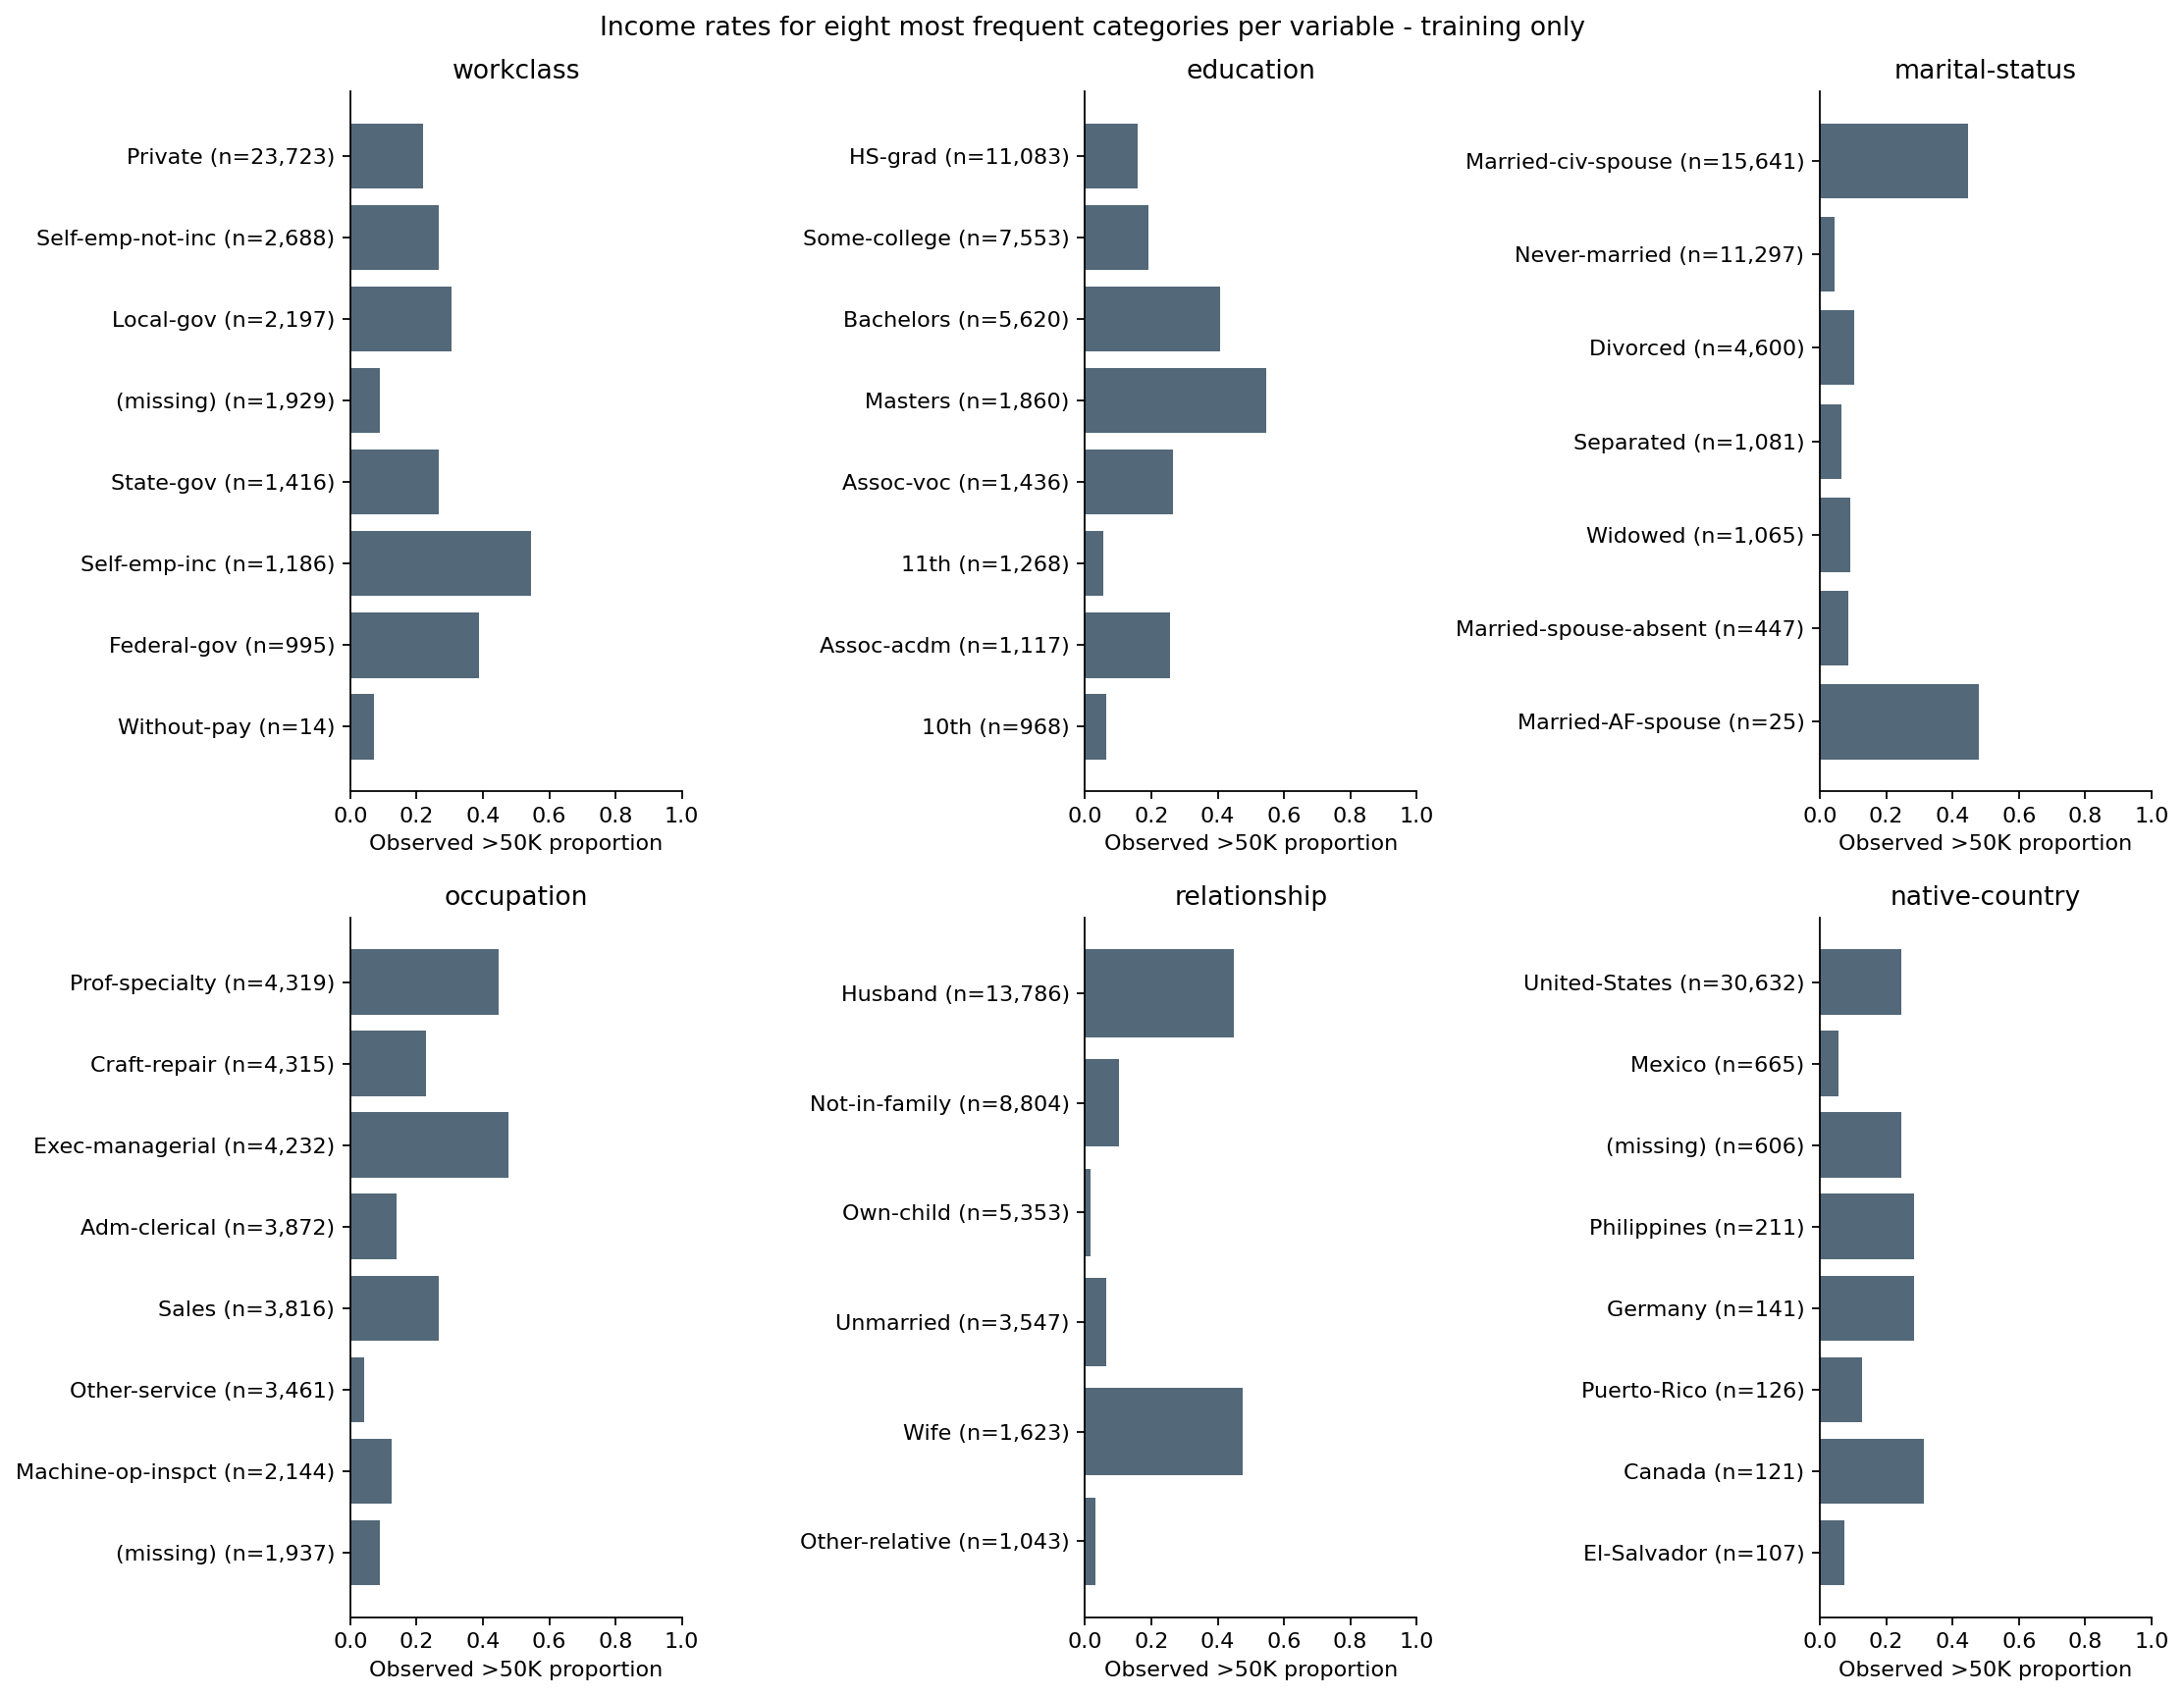
\includegraphics[width=0.86\textwidth]{05_categorical_target_rates.png}
\caption{Part de \texttt{>50K} par modalité (train). Les lignes où \texttt{workclass} ou \texttt{occupation} manque n'ont que 9\,\% de \texttt{>50K}.}
\label{fig:eda}
\end{figure}

%=====================================================================
\section{Ingénierie des variables}

Les 11 prédicteurs retenus passent par une chaîne de quatre étapes (\texttt{census\_income/features.py}) :
\begin{enumerate}
\item \textbf{Imputation} : \texttt{workclass} et \texttt{occupation} manquants deviennent \texttt{"Unemployed"}, \texttt{native-country} manquant devient \texttt{"Unknown"}. C'est une hypothèse métier assumée : ces deux colonnes manquent ensemble, et ces personnes ont un taux de \texttt{>50K} de 9\,\% contre 24\,\% en moyenne (figure~\ref{fig:eda}), ce qui correspond à un profil sans emploi déclaré.
\item \textbf{Catégories rares} : \texttt{Never-worked} et \texttt{Without-pay} sont fusionnées en \texttt{Other} ; \texttt{native-country} est ramené à trois modalités (\texttt{United-States}, \texttt{Other}, \texttt{Unknown}). \texttt{Unknown} reste distinct de \texttt{Other}, pour ne pas confondre « pays non renseigné » et « pays étranger connu ».
\item \textbf{Trois features créées} : \texttt{capital\_gain\_log} et \texttt{capital\_loss\_log} ($\log(1+x)$, qui écrase l'échelle de 0 à 99\,999 pour les modèles linéaires), et \texttt{capital\_gain\_capped}, indicateur du plafond de saisie. Les colonnes brutes sont ensuite retirées pour éviter la redondance.
\item \textbf{Encodage} : standardisation des numériques, one-hot des catégorielles (\texttt{handle\_unknown="ignore"}). On obtient \textbf{50 colonnes}.
\end{enumerate}
Les règles 2 et 3 sont fixes (non apprises) ; l'imputation et l'encodage sont appris dans le \texttt{Pipeline}.

\paragraph{Faut-il garder les colonnes de plus-values ?} Elles sont nulles pour plus de 90\,\% des personnes, mais leurs valeurs non nulles sont parmi les plus prédictives (section~2 ; SHAP les classe au troisième rang, section~7). Une réserve : le revenu cible inclut probablement les plus-values. Une partie des bonnes prédictions vient donc d'un lien presque mécanique avec la cible. Nous les gardons, car le cas d'usage dispose de cette information au moment de prédire, et nous signalons cette limite.

%=====================================================================
\section{Déséquilibre des classes}

\begin{table}[H]
\centering\small
\begin{tabular}{lccccccc}
\toprule
Régression logistique (validation) & AP & ROC-AUC & Précision & Rappel & F1 & TP & FN \\
\midrule
Modèle naïf (toujours \texttt{<=50K}) & 0,239 & 0,500 & 0 & 0 & 0 & 0 & 1\,752 \\
Sans pondération, seuil 0,50 & 0,742 & 0,900 & 0,719 & 0,586 & 0,646 & 1\,026 & 726 \\
\texttt{class\_weight="balanced"}, seuil 0,50 & 0,738 & 0,900 & 0,557 & 0,853 & 0,674 & 1\,494 & 258 \\
\textbf{Sans pondération, seuil 0,282} & \textbf{0,742} & \textbf{0,900} & 0,590 & 0,812 & \textbf{0,683} & 1\,422 & 330 \\
\bottomrule
\end{tabular}
\caption{Effet du remède au déséquilibre (\texttt{census\_income/imbalance.py}).}
\label{tab:imbalance}
\end{table}

Sans remède, la régression logistique est prudente : elle rate 726 des 1\,752 personnes \texttt{>50K}. La pondération des classes fait passer le rappel de 59\,\% à 85\,\%. Mais en validation croisée, l'AP (0,737\,$\pm$\,0,005 contre 0,734\,$\pm$\,0,005) et le ROC-AUC (0,898 dans les deux cas) sont identiques : \textbf{la pondération ne rend pas le modèle meilleur pour distinguer les classes}. En revanche, les écarts de précision et de rappel valent 15 à 20 fois l'écart-type : le compromis est réel. Baisser le seuil du modèle non pondéré à 0,25 reproduit presque exactement le modèle pondéré (0,563 / 0,843 / 0,675). La pondération revient donc surtout à déplacer le seuil, tout en gonflant les probabilités.

\textbf{Remède retenu} : aucune pondération ; pour chaque modèle, un seuil choisi sur la validation pour maximiser le F1 (\texttt{find\_best\_threshold}). Il donne le meilleur F1, laisse le classement intact et garde des probabilités fidèles, utiles pour la calibration (section~8). Les scores mesurés au seuil choisi sur la validation sont légèrement optimistes ; le score définitif est celui du test (section~10).

%=====================================================================
\section{Progression de modélisation}

Trois modèles sont comparés avec le même preprocessing, sur les mêmes 5 découpages groupés (\texttt{census\_income/compare\_models.py}, réglages initiaux fixés avant de voir les résultats).

\begin{table}[H]
\centering\small
\begin{tabular}{lcccccc}
\toprule
Modèle & AP (CV) & ROC-AUC (CV) & F1 à 0,5 (CV) & AP train & Seuil & F1 validation \\
\midrule
Modèle naïf & 0,239 & 0,500 & 0 & -- & -- & 0 \\
Régression logistique & 0,737\,$\pm$\,0,009 & 0,898 & 0,642 & 0,739 & 0,282 & 0,683 \\
Random Forest & 0,804\,$\pm$\,0,003 & 0,917 & 0,686 & 0,912 & 0,435 & 0,717 \\
Gradient Boosting & \textbf{0,824\,$\pm$\,0,003} & \textbf{0,926} & \textbf{0,706} & 0,873 & 0,405 & \textbf{0,731} \\
\bottomrule
\end{tabular}
\caption{Comparaison des trois modèles avant réglage.}
\label{tab:models}
\end{table}

\begin{figure}[H]
\centering
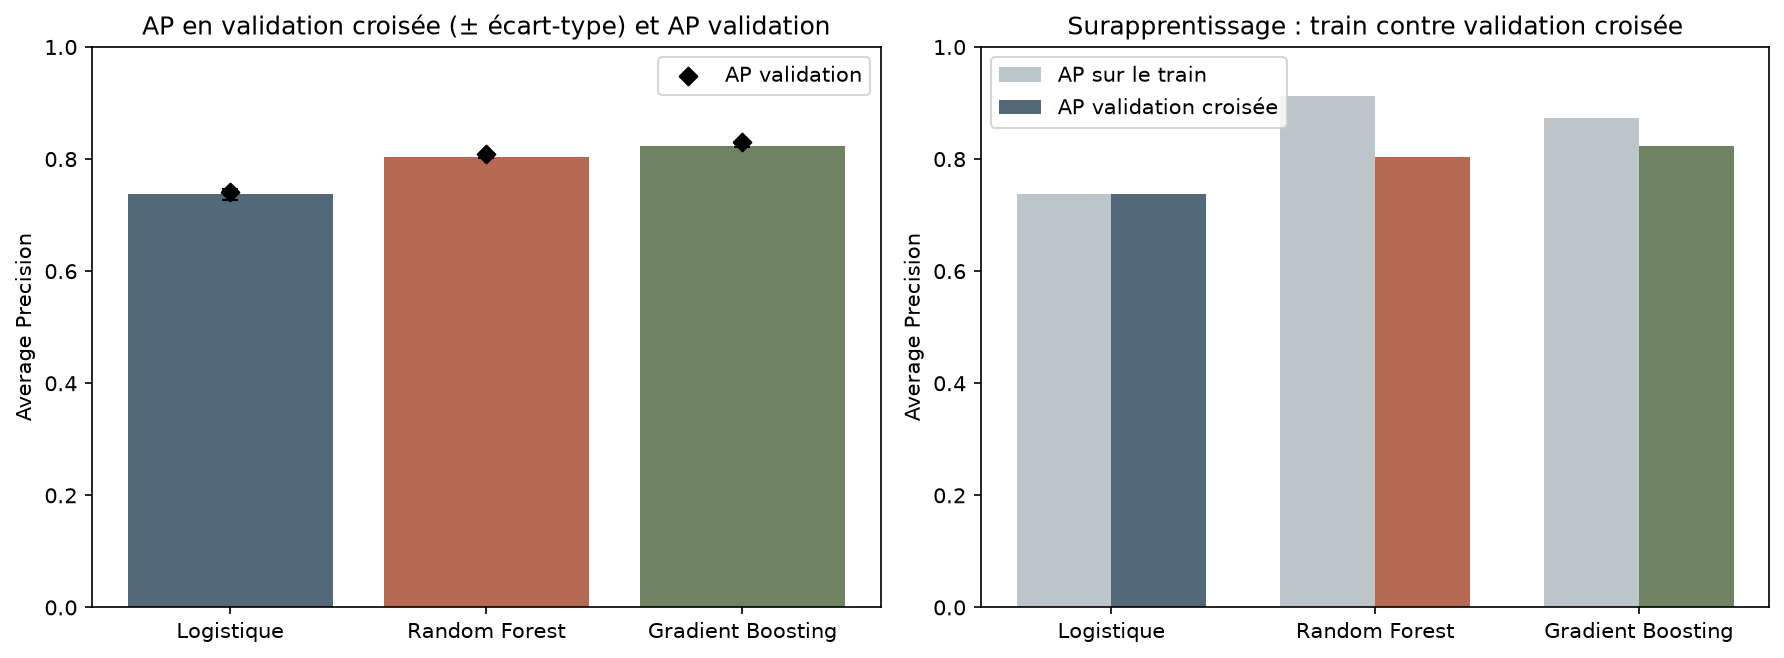
\includegraphics[width=0.95\textwidth]{01_progression_modeles.png}
\caption{AP en validation croisée, et écart entre le score sur le train et en validation croisée (surapprentissage).}
\end{figure}

\begin{itemize}
\item \textbf{Logistique $\rightarrow$ Random Forest : +6,7 points d'AP.} Les arbres captent des interactions (par exemple « marié \emph{et} diplômé \emph{et} plus de 45\,h ») qu'un modèle additif ne voit pas. Contrepartie : un fort surapprentissage (AP de 0,912 sur le train contre 0,804 en validation croisée).
\item \textbf{Random Forest $\rightarrow$ Gradient Boosting : +2 points d'AP}, avec deux fois moins de surapprentissage (écart 0,049 contre 0,107) et un entraînement plus rapide. Les arbres successifs corrigent les erreurs résiduelles de leurs prédécesseurs.
\item La logistique ne surapprend pas (écart 0,002) : elle est limitée par sa forme, pas par la variance.
\end{itemize}

%=====================================================================
\section{Pipeline, réglage Optuna et suivi MLflow}

\paragraph{Pipeline.} Un seul objet \texttt{sklearn.Pipeline} enchaîne imputation, regroupement des catégories rares, features de plus-values, encodage et modèle (\texttt{census\_income/pipeline.py}). C'est cet objet qui est validé, réglé, enregistré (avec son seuil) et servi par l'API.

\paragraph{Réglage.} Optuna (échantillonneur TPE, graine 42) maximise l'AP moyenne en validation croisée groupée, \textbf{sur le train uniquement}. Le premier essai reprend les réglages de la section~5, si bien que le modèle réglé ne peut pas être moins bon que celui de départ. Espaces de recherche : \texttt{C} pour la logistique (25 essais) ; nombre d'arbres, profondeur, taille des feuilles et part des variables pour le Random Forest (20 essais) ; taux d'apprentissage, nombre d'itérations, nombre de feuilles, taille minimale des feuilles, régularisation L2 et part des variables pour le Gradient Boosting (40 essais). La validation, jamais vue pendant la recherche, mesure ensuite les modèles réglés sans biais d'optimisme.

\begin{table}[H]
\centering\small
\begin{tabular}{lcccc}
\toprule
Modèle & AP CV avant & AP CV après & AP validation avant & AP validation après \\
\midrule
Régression logistique & 0,737 & 0,737 & 0,742 & 0,742 \\
Random Forest & 0,804 & 0,809 & 0,809 & 0,818 \\
\textbf{Gradient Boosting} & 0,824 & \textbf{0,827} & 0,831 & \textbf{0,833} \\
\bottomrule
\end{tabular}
\caption{Gain du réglage Optuna (\texttt{census\_income/tuning.py}).}
\end{table}

Les gains sont modestes, ce qui indique que les réglages initiaux étaient déjà raisonnables. Le Random Forest gagne le plus (+0,9 point en validation) en limitant la profondeur à 15. \textbf{Le Gradient Boosting réglé est retenu} (meilleure AP en validation croisée) : taux d'apprentissage 0,035, 500 itérations, 21 feuilles, 40 observations minimum par feuille, 62\,\% des variables par arbre. Son seuil, choisi sur la validation, vaut \textbf{0,404} (F1 de validation 0,736).

\paragraph{Suivi des expériences.} Chaque essai Optuna est une exécution MLflow (85 au total), qui enregistre les réglages, l'AP moyenne et son écart-type, le ROC-AUC, le F1 et la durée. Chaque modèle a aussi une exécution « parent » qui garde les meilleurs réglages et le tableau de tous les essais ; une dernière exécution enregistre le modèle final, son seuil et ses métriques (base \texttt{mlflow.db}, consultable avec \texttt{mlflow ui} ; les 89 exécutions sont exportées dans \texttt{reports/tuning/mlflow\_runs.csv}).

%=====================================================================
\section{Explicabilité (SHAP)}

Les valeurs SHAP du modèle final sont calculées par \texttt{TreeExplainer} sur 1\,000 personnes de la validation. Elles sont exprimées en log-odds : une valeur positive pousse vers \texttt{>50K}. Pour l'importance globale par variable d'origine, les colonnes one-hot d'une même variable sont additionnées pour chaque personne avant de prendre la valeur absolue.

\begin{figure}[H]
\centering
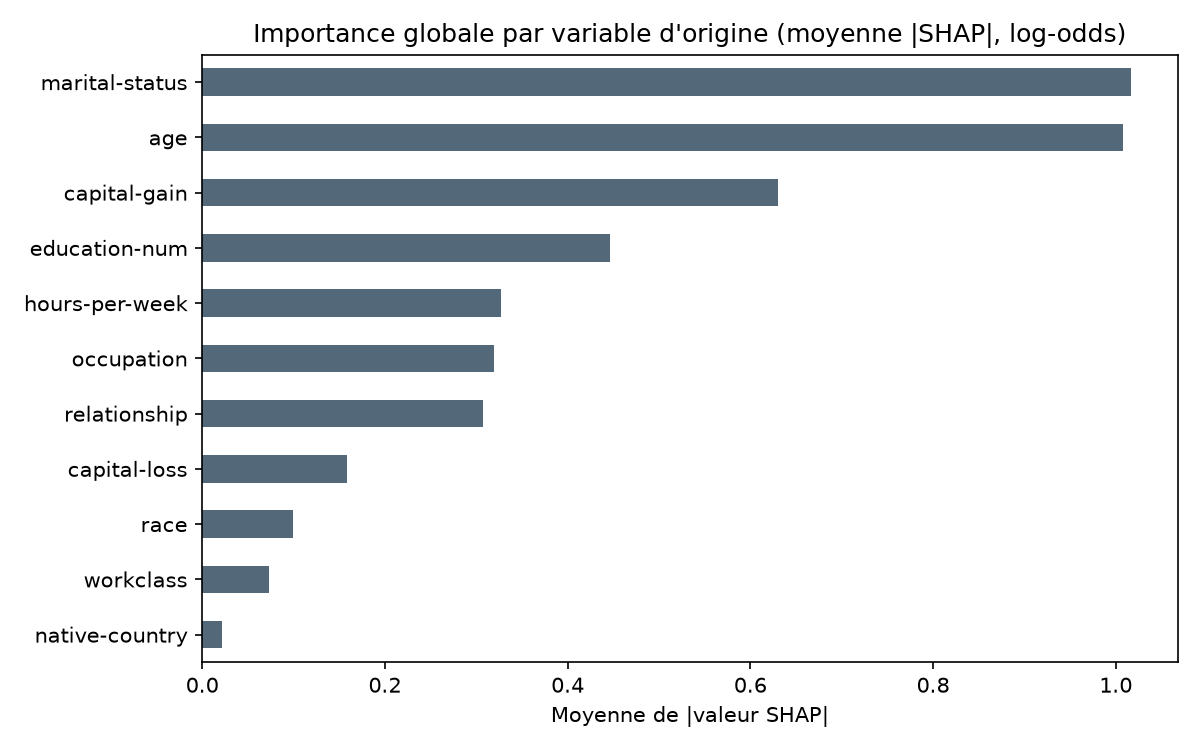
\includegraphics[width=0.49\textwidth]{02_importance_par_variable.png}\hfill
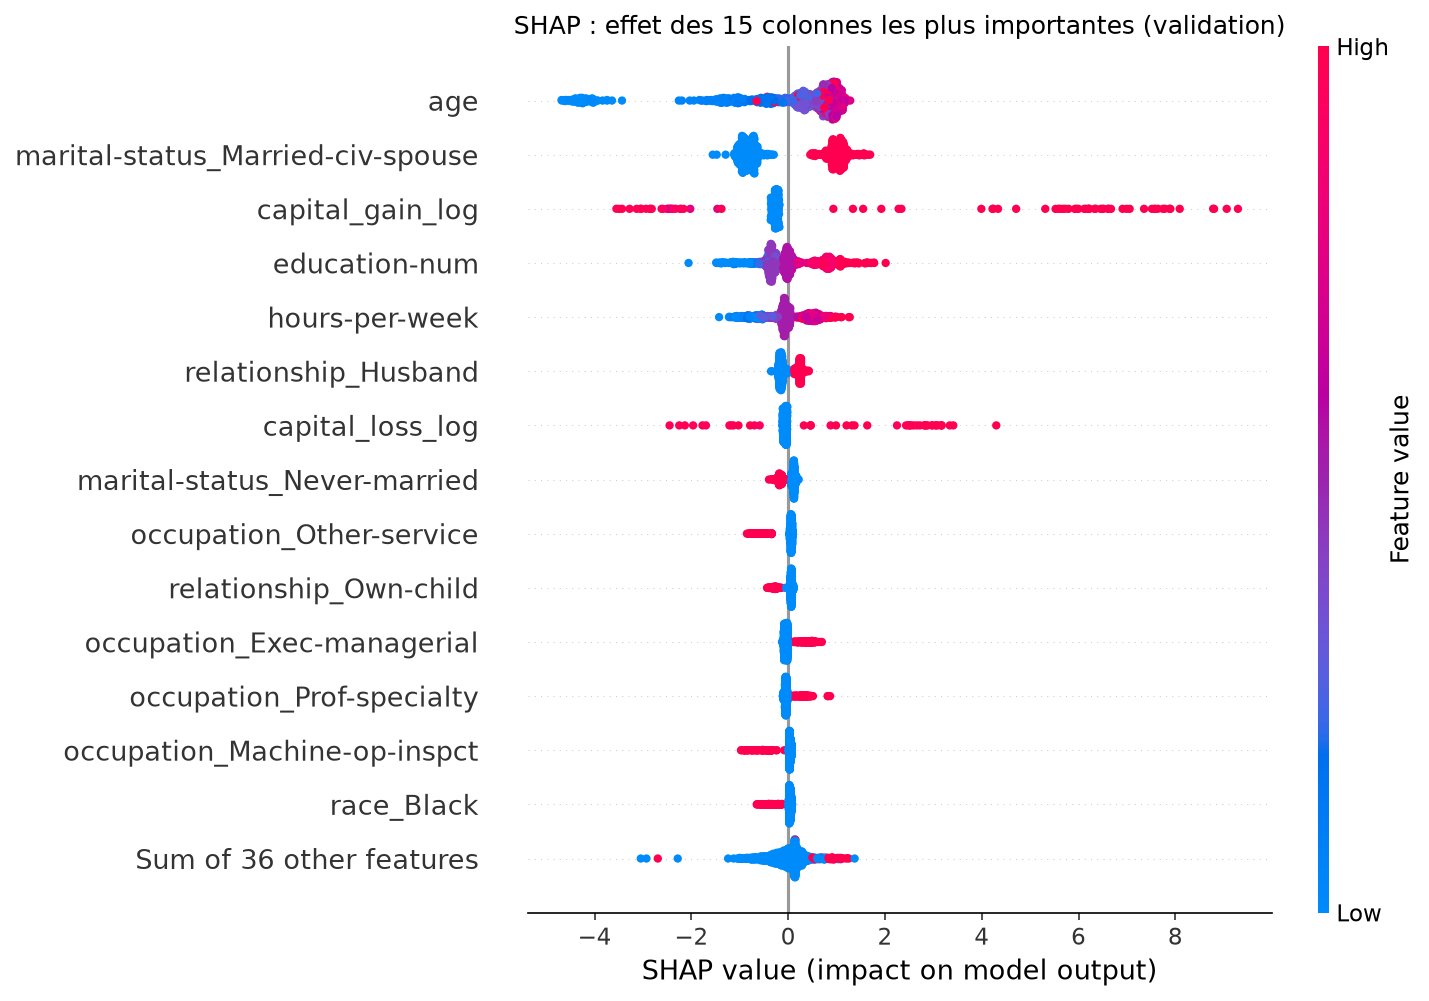
\includegraphics[width=0.49\textwidth]{01_shap_beeswarm.png}
\caption{Importance globale par variable d'origine (gauche) et effet des colonnes les plus importantes (droite).}
\end{figure}

\paragraph{Les variables importantes ont-elles un sens métier ?} Oui, dans l'ensemble :
\begin{itemize}
\item \textbf{Statut marital et âge} dominent (1,02 et 1,01). Être marié augmente fortement la probabilité ; c'est une association (liée à l'âge, à la stabilité professionnelle et aux normes de déclaration de l'époque), pas un effet causal du mariage. Les plus jeunes sont très pénalisés, et l'effet de l'âge devient positif aux âges de pleine carrière.
\item \textbf{Plus-values} (0,63) : les plus-values élevées poussent très fort vers \texttt{>50K}, mais les petites plus-values (moins de 5\,000\,\$) font \emph{baisser} la probabilité. Le modèle a retrouvé seul le constat de l'EDA (17,9\,\% de \texttt{>50K} dans cette tranche).
\item \textbf{Niveau d'études, heures travaillées et profession} (cadres et professions intellectuelles vers le haut, services et ouvriers vers le bas) suivent l'intuition économique.
\item \textbf{Point de vigilance} : \texttt{relationship} (\texttt{Husband}) et \texttt{race\_Black} ont un effet propre. \texttt{relationship} est un proxy du sexe, ce qui explique qu'exclure \texttt{sex} ne suffise pas à rendre le modèle équitable (section~9).
\end{itemize}

\begin{figure}[H]
\centering
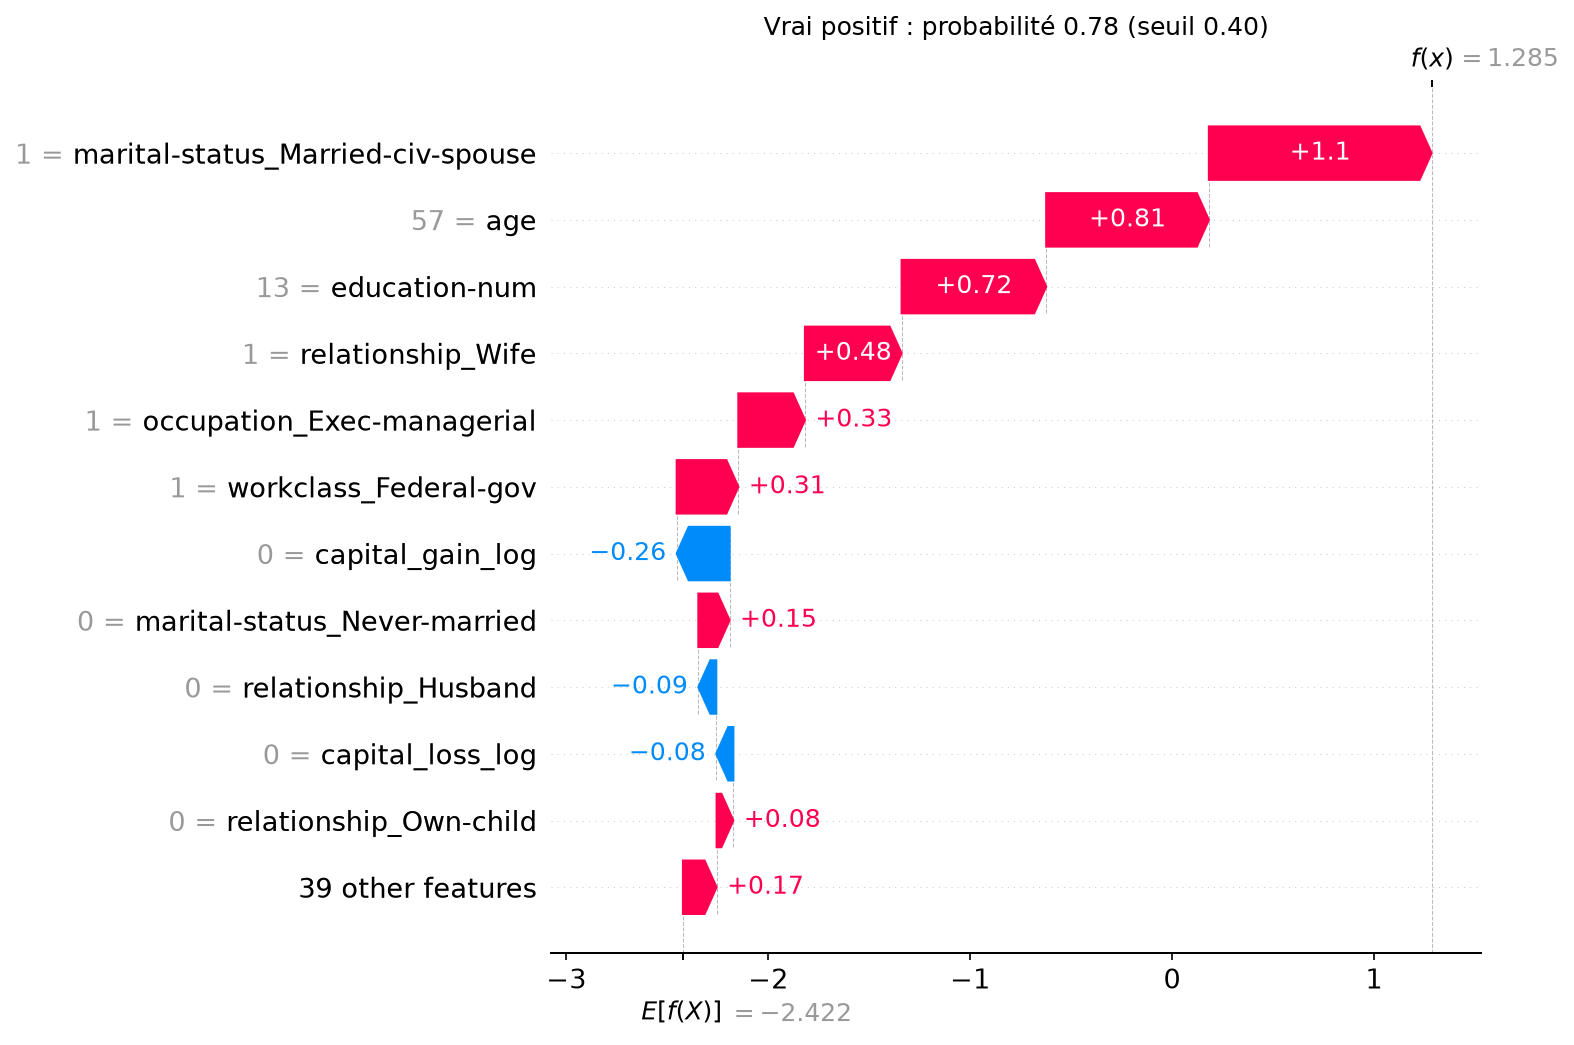
\includegraphics[width=0.49\textwidth]{03_local_vrai_positif.png}\hfill
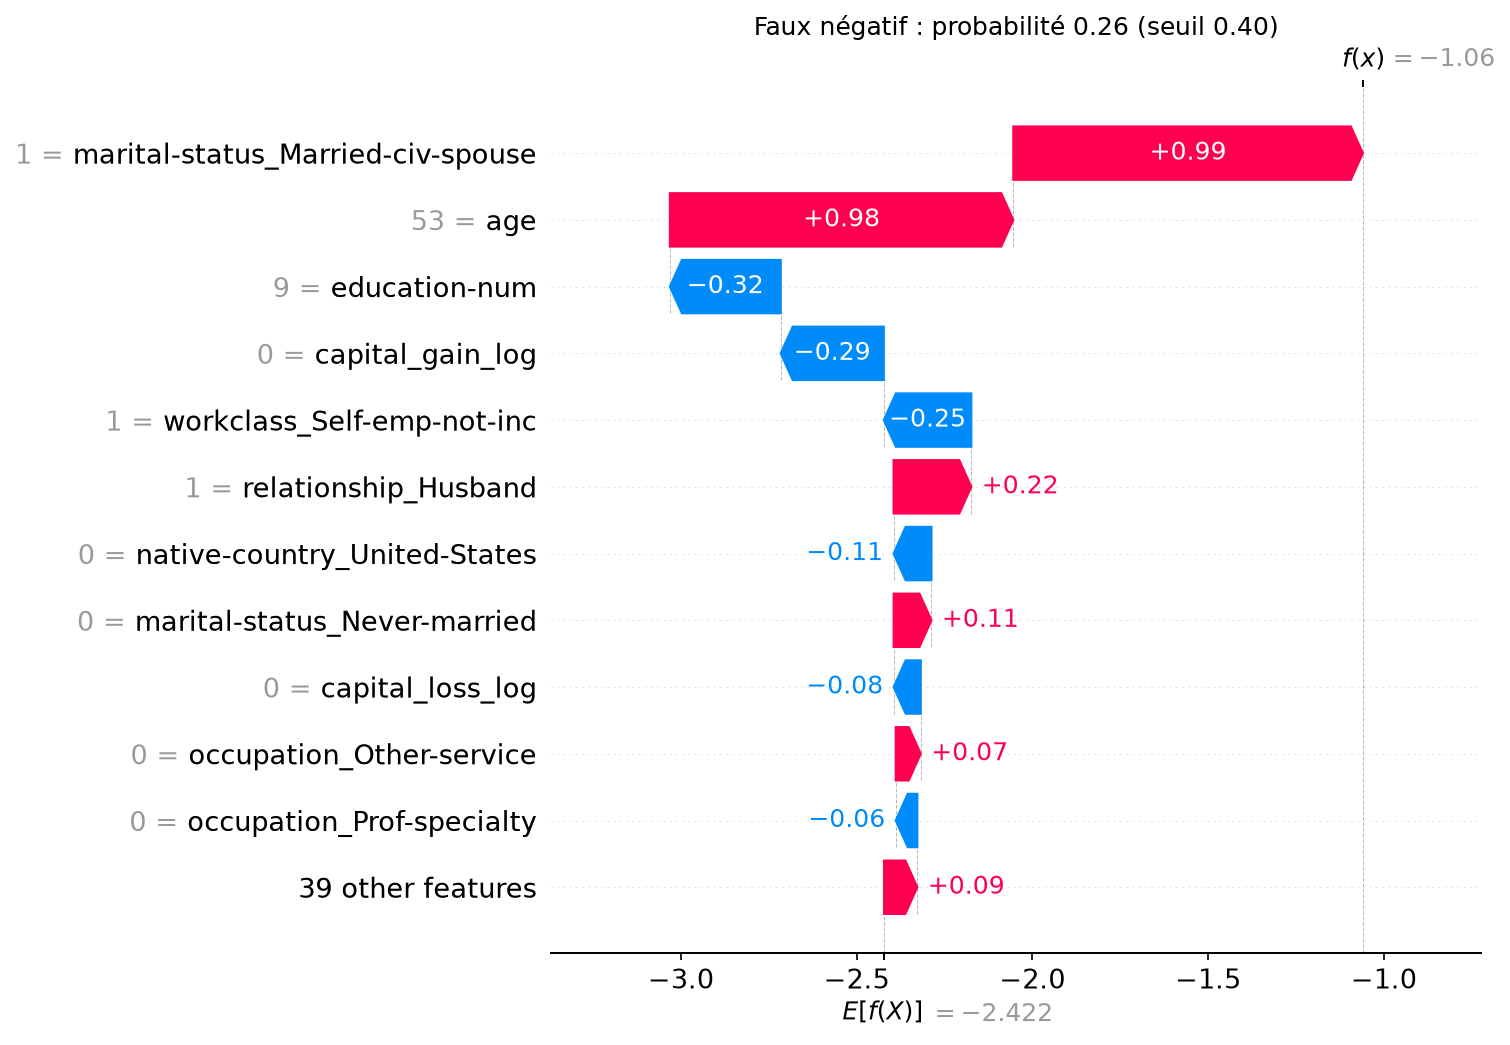
\includegraphics[width=0.49\textwidth]{04_local_faux_negatif.png}
\caption{Explications locales : un vrai positif (gauche, probabilité 0,78) et un faux négatif (droite, 0,26).}
\end{figure}

\paragraph{Explications locales.} Quatre personnes, une par case de la matrice de confusion, sont expliquées (\texttt{reports/explainability/}). La femme de 57 ans, cadre de la fonction publique fédérale, mariée et titulaire d'une licence, est un vrai positif (0,78) : statut marital, âge et diplôme s'additionnent. Le faux négatif est un homme de 53 ans, marié, travailleur indépendant dans l'artisanat, sans diplôme du supérieur ni plus-value. Statut marital et âge le poussent vers le haut, mais le niveau d'études, l'absence de plus-value et le statut d'indépendant le ramènent à 0,26. C'est un profil où le revenu dépend de facteurs absents des données (chiffre d'affaires de l'activité). Le faux positif (0,54) est un homme de 49 ans, marié, agent de la fonction publique locale (services de protection), sans diplôme du supérieur : son profil ressemble à celui des hauts revenus mariés sans en avoir le revenu. Le vrai négatif (0,02) a 50 ans, n'a jamais été marié, est peu diplômé et travaille 25\,h par semaine.

%=====================================================================
\section{Calibration}

\begin{figure}[H]
\centering
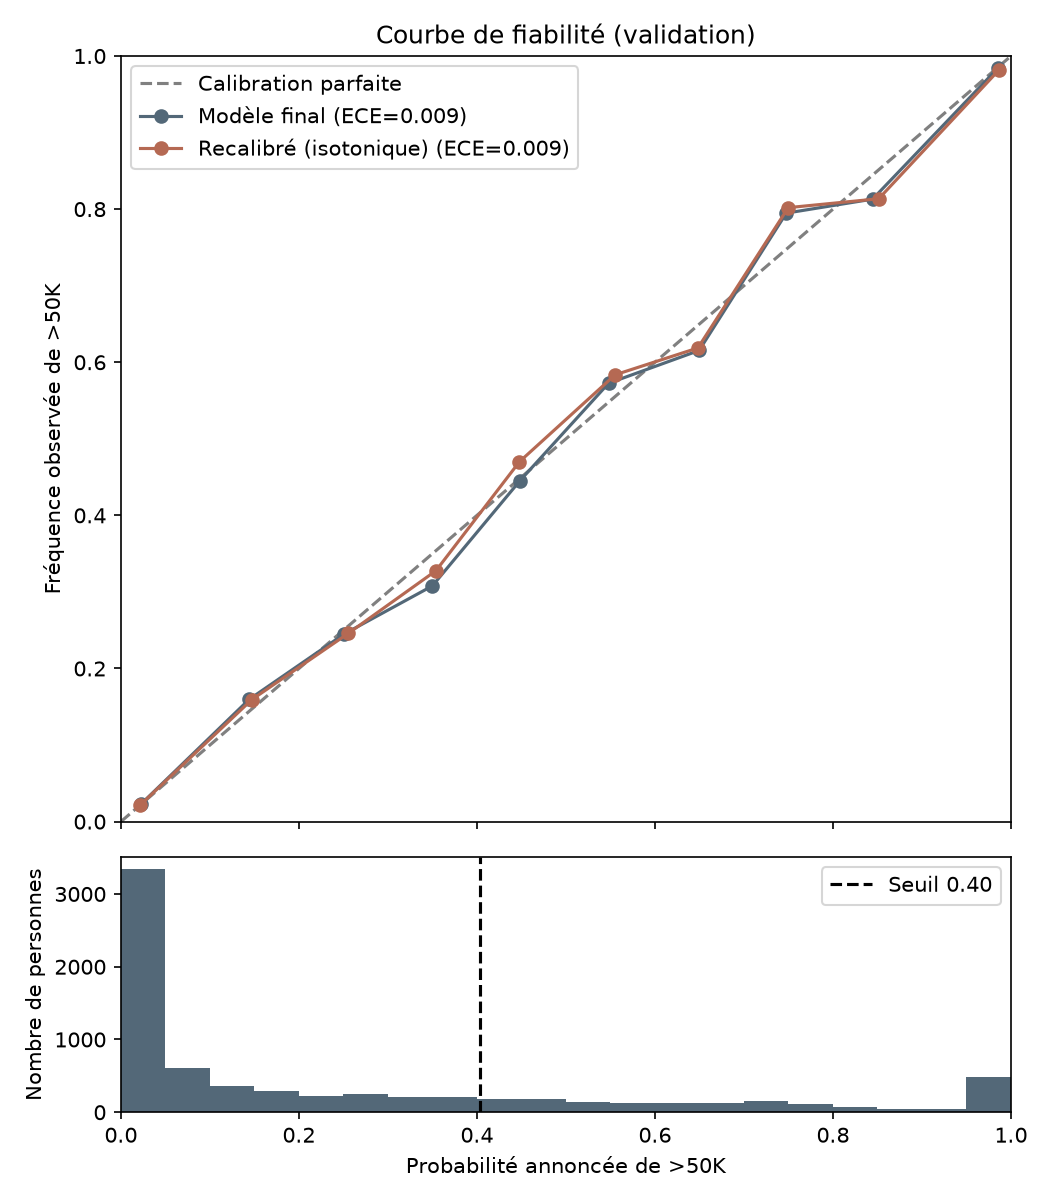
\includegraphics[width=0.52\textwidth]{01_courbe_fiabilite.png}
\caption{Courbe de fiabilité du modèle final sur la validation (10 tranches) et distribution des probabilités.}
\end{figure}

\begin{table}[H]
\centering\small
\begin{tabular}{lccc}
\toprule
Validation & Brier & ECE & Écart signé \\
\midrule
Modèle final (Gradient Boosting) & \textbf{0,087} & \textbf{0,009} & +0,001 \\
Même modèle recalibré (isotonique, CV sur le train) & 0,087 & 0,009 & +0,000 \\
Référence : toujours la proportion de \texttt{>50K} & 0,182 & 0,000 & 0,000 \\
\bottomrule
\end{tabular}
\caption{Diagnostic de calibration (\texttt{census\_income/calibration.py}).}
\end{table}

La courbe suit la diagonale. L'écart moyen entre probabilité annoncée et fréquence observée (ECE) est inférieur à un point. Le Brier score (0,087) est deux fois plus faible que celui de la référence constante (0,182). Cette référence a un ECE nul, ce qui rappelle qu'une bonne calibration ne suffit pas : il faut aussi discriminer. Les écarts par tranche restent sous 5 points et changent de signe : \textbf{le modèle n'est ni sur-confiant ni sous-confiant de façon notable}, et une recalibration isotonique n'apporte rien. C'est cohérent avec l'absence de pondération des classes, qui aurait gonflé les probabilités. \textbf{Nous ferions confiance à ces probabilités telles quelles} pour une décision en aval, sur une population comparable à celle de 1994. Un usage sur d'autres données demanderait de revérifier la calibration.

%=====================================================================
\section{Équité}

L'attribut sensible est \texttt{sex}. Il n'est pas utilisé comme prédicteur, mais des proxys (\texttt{relationship}, \texttt{marital-status}) restent présents. Nous suivons deux définitions :
\begin{itemize}
\item \textbf{la parité démographique} : même taux de prédiction \texttt{>50K} dans les deux groupes ;
\item \textbf{l'égalité des chances} (equal opportunity) : même rappel, c'est-à-dire qu'une personne réellement \texttt{>50K} a la même chance d'être reconnue, qu'elle soit une femme ou un homme.
\end{itemize}
Les taux réels de \texttt{>50K} diffèrent fortement (10,7\,\% contre 30,8\,\% sur le test) : la parité démographique exigerait de prédire autant de hauts revenus chez les femmes que chez les hommes, malgré des taux réels très différents. Nous visons donc l'égalité des chances.

\paragraph{Atténuation.} Nous appliquons un post-traitement : un seuil par groupe (méthode de Hardt et al., 2016). Les seuils sont choisis sur la validation pour que chaque groupe atteigne le rappel global (0,744) : 0,295 pour les femmes, 0,415 pour les hommes. Ils sont ensuite appliqués tels quels au test intact.

\begin{table}[H]
\centering\small
\begin{tabular}{lcccccc}
\toprule
Test & \multicolumn{2}{c}{Rappel (TPR)} & \multicolumn{2}{c}{Taux de sélection} & \multicolumn{2}{c}{Précision} \\
 & Femmes & Hommes & Femmes & Hommes & Femmes & Hommes \\
\midrule
Avant (seuil unique 0,404) & 0,647 & 0,767 & 0,095 & 0,329 & 0,728 & 0,719 \\
Après (seuils par groupe) & 0,751 & 0,759 & 0,125 & 0,320 & 0,643 & 0,730 \\
\bottomrule
\end{tabular}

\vspace{6pt}
\begin{tabular}{lccccc}
\toprule
Test & F1 & Précision & Rappel & Écart de rappel & Écart de parité démographique \\
\midrule
Avant & 0,734 & 0,720 & 0,749 & 0,121 & 0,233 \\
Après & 0,736 & 0,715 & 0,757 & \textbf{0,008} & 0,195 \\
\bottomrule
\end{tabular}
\caption{Audit d'équité par sexe sur le test, avant et après atténuation (\texttt{census\_income/fairness.py}).}
\end{table}

\begin{figure}[H]
\centering
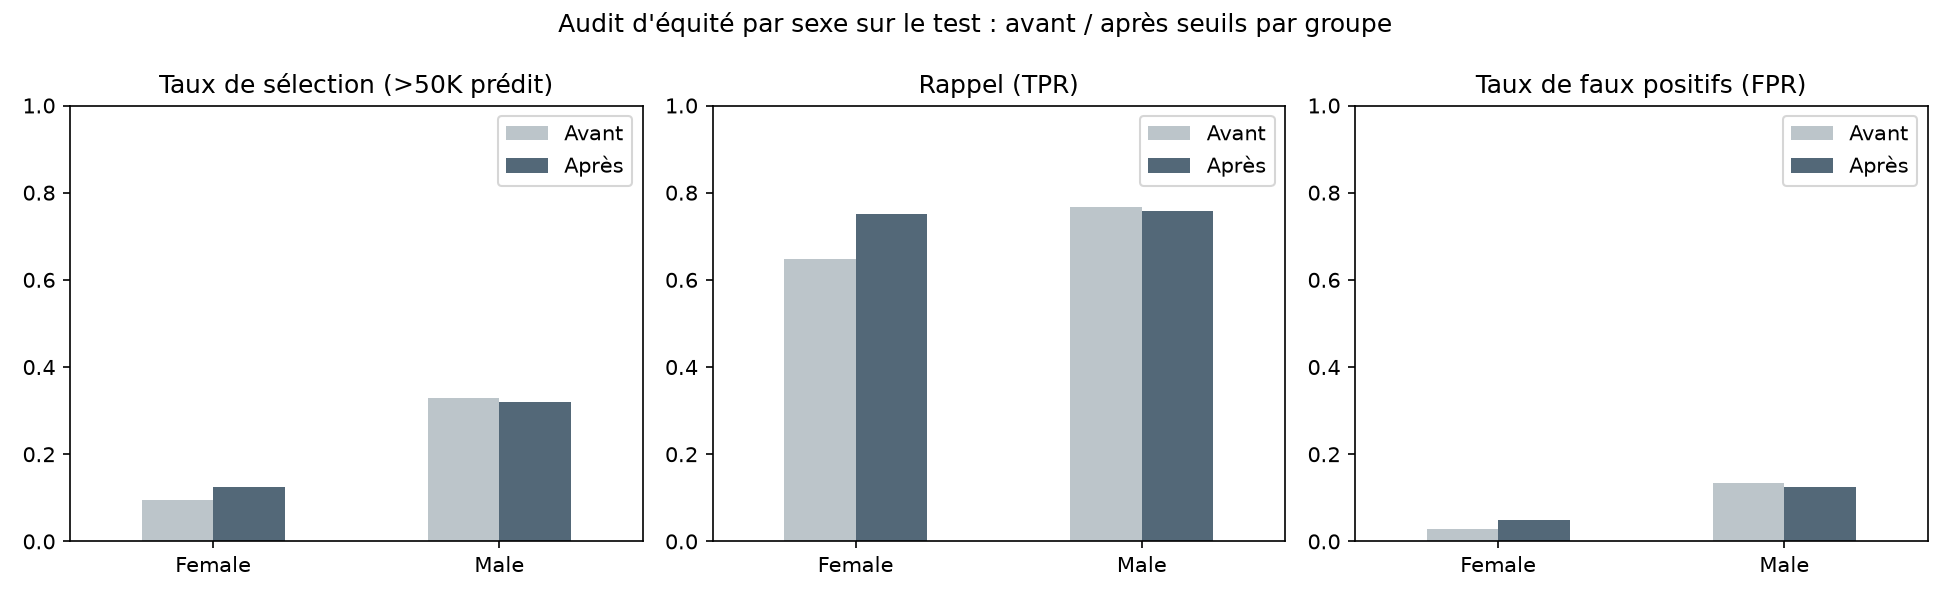
\includegraphics[width=0.92\textwidth]{01_equite_avant_apres.png}
\caption{Taux de sélection, rappel et taux de faux positifs par sexe, avant et après atténuation (test).}
\end{figure}

Avant atténuation, une femme réellement \texttt{>50K} n'est reconnue que dans 65\,\% des cas, contre 77\,\% pour un homme. Après atténuation, \textbf{l'écart de rappel passe de 12,1 à 0,8 point, sans perte de performance globale} (F1 de 0,734 à 0,736). L'écart de parité démographique diminue aussi, mais reste élevé (0,195), car il reflète en grande partie l'écart des taux réels. Le coût est porté par la précision chez les femmes (0,728 à 0,643) : davantage de fausses alertes, ce qui illustre le compromis entre définitions d'équité. Limite importante : cette méthode utilise le sexe au moment de la décision. Selon le contexte juridique, ce traitement différencié peut être interdit ; une méthode en cours d'entraînement (par exemple \texttt{ExponentiatedGradient}) serait alors préférable.

%=====================================================================
\section{Évaluation finale, mise à disposition et limites}

\paragraph{Test.} Évalué une seule fois avec le modèle et le seuil figés, le modèle final obtient \textbf{AP 0,833, ROC-AUC 0,931, précision 0,720, rappel 0,749, F1 0,734, accuracy 0,870, Brier 0,087}. Ces scores sont quasiment identiques à ceux de la validation (AP 0,833, F1 0,736). Le choix du seuil sur la validation n'a donc pas créé d'optimisme visible, et le modèle généralise.

\paragraph{Endpoint.} Le modèle final (Pipeline et seuil) est enregistré avec \texttt{joblib} et servi par une API FastAPI (\texttt{census\_income/api.py}). La route \texttt{POST /predict} reçoit les 11 informations d'une personne et renvoie la probabilité de \texttt{>50K}, le seuil et la prédiction ; \texttt{/predict/batch}, \texttt{/model} et \texttt{/health} complètent l'API. Les entrées sont validées (types, bornes), et les valeurs manquantes sont acceptées et imputées par le Pipeline. 30 tests automatisés couvrent le découpage, les features, les métriques, les modèles, les étapes finales et l'API.

\paragraph{Limites.}
\begin{itemize}
\item Données de 1994, non pondérées par \texttt{fnlwgt} : les résultats décrivent l'échantillon, pas la population américaine actuelle.
\item Associations prédictives, pas causales : l'effet du statut marital ne signifie pas que le mariage augmente le revenu.
\item Lien quasi mécanique entre plus-values et revenu cible ; hypothèse « Unemployed » pour les valeurs manquantes.
\item Atténuation fondée sur le sexe au moment de la décision ; l'origine (\texttt{race}) n'a pas été auditée ni corrigée.
\item L'EDA initiale a porté sur la table complète, test compris (choix descriptifs uniquement).
\end{itemize}

\paragraph{Conclusion.} Le Gradient Boosting réglé, sans pondération et avec un seuil choisi sur la validation, offre le meilleur compromis : AP de 0,833 sur le test, des probabilités bien calibrées et des explications cohérentes avec l'intuition économique. Un post-traitement simple corrige l'écart de rappel entre femmes et hommes sans coût global.

%=====================================================================
\section*{Contributions}
\begin{tabularx}{\textwidth}{lX}
\toprule
Membre & Rôle \\
\midrule
Jérémy Caillaud & EDA initiale et premiers éléments de cadrage (notebook \texttt{01\_eda}) ; guide Git de l'équipe. \\
Hugo van Zuylen & Cadrage et protocole de validation ; nettoyage et découpage reproductible avec empreintes et tests (\texttt{data.py}, \texttt{explore.py}) ; comparaison des trois modèles en partie 4 (notebook \texttt{04\_model\_comparison}). \\
Yanis Rajhi & Ingénierie des variables (partie 2) ; déséquilibre des classes et métriques communes (partie 3) ; réorganisation du dépôt et conversion de la partie 4 en script ; Pipeline, Optuna, MLflow, SHAP, calibration, équité, endpoint FastAPI et documentation (parties 5 à 10). \\
\bottomrule
\end{tabularx}

\section*{Usage d'assistants IA}
Des assistants IA ont été utilisés tout au long du projet. Claude (Anthropic) a servi à expliquer les notions, à écrire et relire le code (scripts \texttt{census\_income/}, tests, API), à réorganiser le dépôt, à rédiger la documentation et une première version de ce rapport. Une partie des contributions d'EDA, de découpage et de comparaison de modèles a aussi été préparée avec une assistance IA, comme l'indiquent les documents de \texttt{docs/contributions/}. Les choix méthodologiques (métrique principale, remède au déséquilibre, sélection du modèle, définition d'équité) ont été discutés et validés par le groupe ; tous les résultats rapportés proviennent de l'exécution du code du dépôt.

\appendix
\section{Reproduire les résultats}
Depuis la racine du dépôt, après \texttt{pip install -r requirements.txt} :
\begin{verbatim}
python -m census_income.data            # découpage 70/15/15
python -m census_income.compare_models  # partie 4
python -m census_income.tuning          # parties 6-7 (~30 min)
python -m census_income.train_final     # modèle final + seuil
python -m census_income.interpret       # SHAP
python -m census_income.calibration     # calibration
python -m census_income.fairness        # test + équité
uvicorn census_income.api:app           # endpoint
python -m unittest discover -s tests    # 30 tests
\end{verbatim}

\begin{figure}[H]
\centering
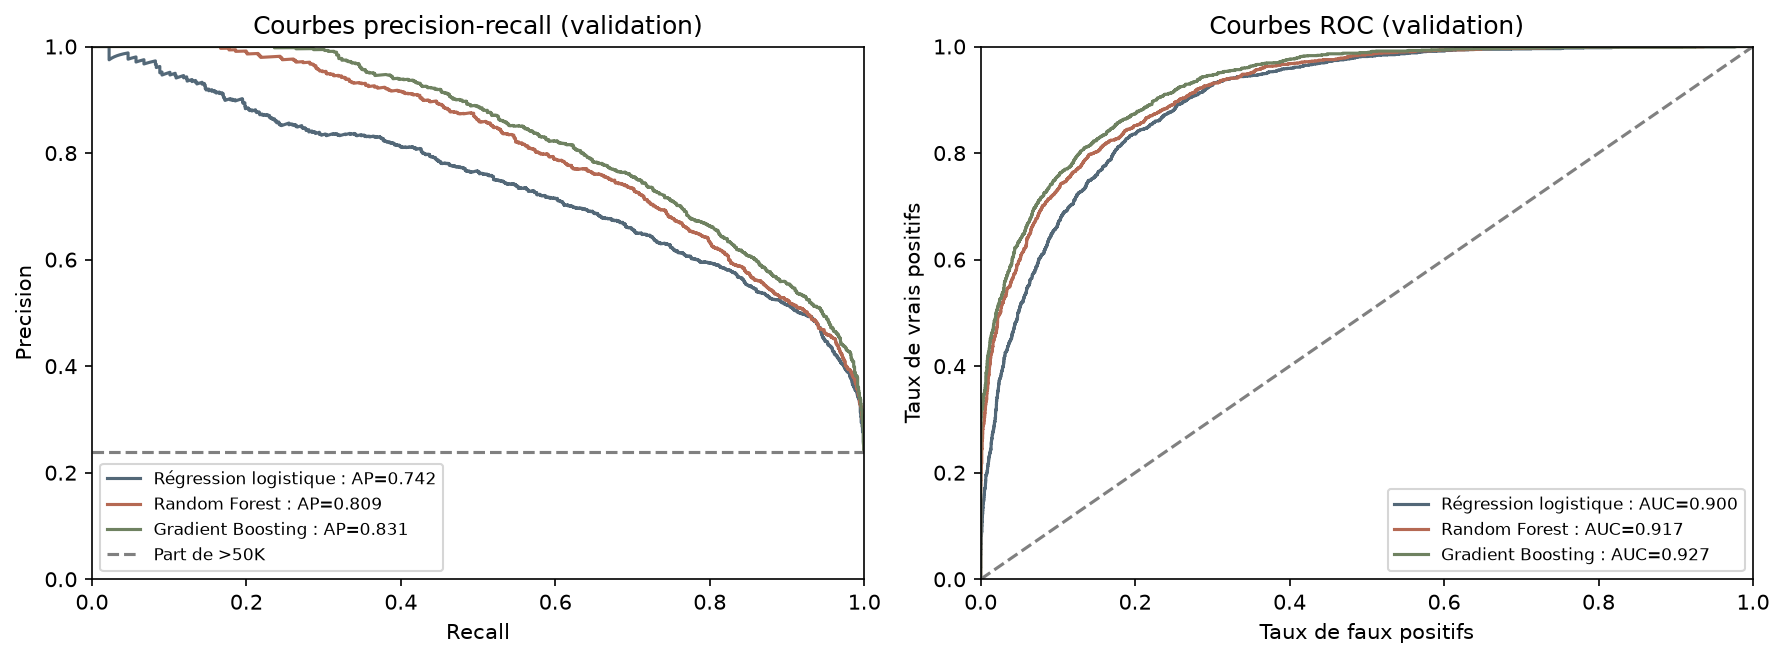
\includegraphics[width=0.9\textwidth]{02_courbes_validation.png}
\caption{Courbes précision-rappel et ROC des trois modèles (validation, avant réglage).}
\end{figure}

\end{document}
